\documentclass[a4paper, 10pt]{article}
\usepackage{pgf}
\usepackage{eurosym}
\usepackage{graphicx}
\usepackage{wasysym}
\usepackage{hyperref}
\usepackage{listings}
\usepackage{pxfonts}
\usepackage{verbatim}
\usepackage{color}
\usepackage{xcolor}
\usepackage{wrapfig}
\usepackage{enumitem}
\usepackage{booktabs}

\hypersetup{
    bookmarks=true,         % show bookmarks bar?
    unicode=true,          % non-Latin characters in Acrobat’s bookmarks
    pdftoolbar=true,        % show Acrobat’s toolbar?
    pdfmenubar=true,        % show Acrobat’s menu?
    pdffitwindow=true,     % window fit to page when opened
    pdftitle={Practical Exercises},    % title
    pdfauthor={Paul Vesey},     % author
    pdfsubject={Project Management},   % subject of the document
    pdfcreator={},   % creator of the document
    pdfproducer={xelatex}, % producer of the document
    pdfkeywords={'Project Management' }, % list of keywords
    pdfnewwindow=true,      % links in new PDF window
    colorlinks=true,       % false: boxed links; true: colored links
    linkcolor=violet,          % color of internal links (change box color with linkbordercolor)
    citecolor=magenta,        % color of links to bibliography
    filecolor=red,      % color of file links
    urlcolor=blue           % color of external links
}

\setlength\parindent{0pt}
\begin{document}

\lstset{language=HTML,
				basicstyle=\small,
				breaklines=true,
        numbers=left,
        numberstyle=\tiny,
        showstringspaces=false,
        aboveskip=-20pt,
        frame=leftline
        }
				
\begin{table}%
	\begin{minipage}{0.4\textwidth}%
			
\includegraphics[width=1\textwidth]{img/LITlogo.jpg}
	\end{minipage}
	\qquad
	\centering
	\parbox{0.4\textwidth}{
		\begin{large}			
			\begin{tabular}{| r | l |} \hline
				Subject: & \textbf{Web Development}\\
				Course: & \textbf{HDip in Software Development}\\
				Session: & \textbf{2017-2018}\\
				Lecturer: & \textbf{Paul Vesey \footnotesize{BEng, MIE, HDip}}\\
				\hline
			\end{tabular}
		\end{large}			
	}
\end{table}
\vspace{0.25cm}	
	
\begin{flushleft}
\Large\textbf{Assignment 2 (25\%)- Static HTML Website with CSS}\\
\end{flushleft}

In this assignment you are required to design and develop a 5 page static HTML website that utilizes one or more external CSS files and a Grid system of your own creation\footnote{Use of commercial, free, and/or open source systems is expressly forbidden}. The key deliverables for this project are:

\begin{enumerate}
	\item Pencil Project Wire-frame Design of Grid system
	\item Pencil Project Wire-frame Design for all pages
	\item Five Page Website, styled with external CSS file(s)
	\item W3C Validated HTML and CSS
	\item Detailed Report on the design process and how the site fulfills the design objective described below.
\end{enumerate}


\textbf{Background}\\

% (2013-2014) You are required to develop a website to promote the art of Joan Mir\'{o} (1893-1983).  Mir\'{o} was 20$^{th}$ century painter and sculptor of considerable note.  His style developed through several schools including fauvism, realism and surrealism.  A consistent characteristic of his work was his use of color, in particular strong primary colors.  One of my favorite works is his collection of illustrated poems commonly known as 'Parler Seul'.\\
%You are required to develop a website to promote horology; specifically mechanical wrist watches (manual or automatic winding) from the 1960's to present day.  Mechanical watches went into major decline upon the development of quartz watches in the 1970's and 1980's; this period is known in the industry as the Quartz Crisis.  Since then mechanical watches have undergone a revival as high end luxury item.  Brands to look for are Omega, IWC, Breitling, Jaeger-LeCoultre, and A. Lange \& S\"{o}hne.  The Harry Winston Opus series are also worth investigating.\\

% (2015-2016)You are required to develop a website to promote manual focus, wet process photography; specifically Nikon or Canon manual focus cameras from the 1960's to present day.  Traditional film cameras went into major decline upon the development of digital photography. However, there remains a dedicated following for traditional wet process photography.  \\  

You are required to develop a website to promote Lebanese food to an Irish audience.\\  

\textbf{Key Design Objective}\\

% (2013-2014)Showcase the work of Joan Mir\'{o} and introduce the artist to a new, younger, audience.  You will need to include biography, details of past exhibitions, and reviews.  Use images, audio and video to reinforce your message where necessary.\\

%http://www.laurahampson.com/index.html
%http://www.laurahampson.com/coursework/

% (2015-2016)The site should be targeted at people under 35 years looking for something different or more traditional.  Your objective is to educate and sell film cameras to them.  Your core message should be that image creation takes time, and old cameras will teach you how.  You should also present site visitors with useful resource links for film, chemical and paper. Use images, audio and video to reinforce your message where necessary.\\

The site should be targeted at people under 35 years looking for something different or something considered unusual.  Your objective is to attract and educate site visitors on the diverse nature of Lebanese food.  Your core message should be 'Exciting, Exotic, and Affordable'.  You should also present site visitors with useful resource links for recipes, restaurants, and reviews. Use images, audio and video to reinforce your message where necessary.\\

\textbf{Site Content \& Structure}

\begin{itemize}
	\item Text - At least one sentence to describe what the article or paragraph will contain.  Remaining sentences may be filled out with Lorem Ipsum, but use a variety of extracts from Lorem.
	\item Images - Each image used must be listed in your report, along with the licensing and source information.   
	\item Video \& Audio - All video \& audio must be licensed under creative commons or similar open licensing system.  Each video and audio clip used must be listed in your report, along with the licensing and source information.
	\item Your website is to have a logical folder structure, with separate folders for images, audio, video, wireframe diagrams, and css files. 
\end{itemize}


\vspace{1cm}
\begin{figure}[h!t]
	\centering
	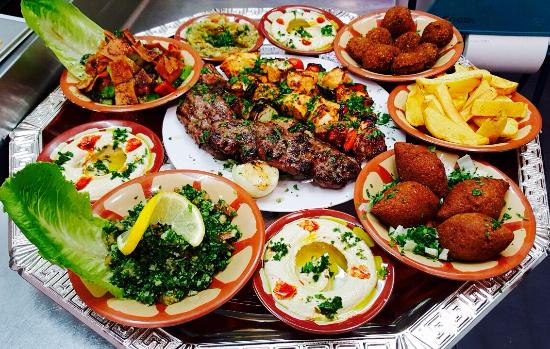
\includegraphics[width = 11cm]{img/lebFood1.jpg}
	\caption{Lebanese Dishes}
	\label{fig:nikonf3}
\end{figure}

\textbf{Report}\\
Your report should be laid out in a professional manner, as would be done for a client.  This involves, \emph{inter-alia}, a cover page, table of contents, and logical sectioning.  Your report should include wireframe images, website screen shots, and other details necessary to communicate design intent.
\vspace{1cm}

\textbf{Submission}\\
Your completed website and documentation are to be zipped into a single file\footnote{Your zip file must preserve your folder structure} and uploaded to Moodle on or before the date and time indicated.  You will be asked to demonstrate the site and explain its operation to your lecturer during class time following submission.




\vspace{1cm}
\begin{figure}[h!t]
	\centering
	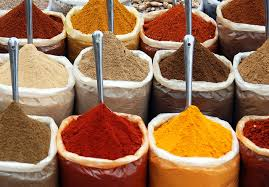
\includegraphics[width = 11cm]{img/lebFood2.jpg}
	\caption{Lebanese Spices}
	\label{fig:reverso}
\end{figure}



\textbf{Late Submission}\\
Failure to submit your assignment on or before the date and time indicated on Moodle will result in a penalty of 5\% per day or part thereof.

\vspace{0.5cm}
\newpage
\textbf{Marking Scheme}\\


\begin{table}[h!]
     \begin{center}
     \begin{tabular}{p{5cm}  p{5cm} }
     \toprule
      \textbf\large{Element} & \textbf\large{Proportion} \\ 
    \cmidrule(r){1-1}\cmidrule(lr){2-2}
      \textbf{Report}
		      \begin{itemize}[topsep=0pt]
		      		\item[] Wireframes
		      		\item[] Report 
		      \end{itemize}
      \textbf{Website}
            	\begin{itemize}[topsep=0pt]
			      \item[] Usability \emph{et. al.}
			      \item[] Design Aesthetic
			      \item[] Responsive Design
			      \item[] Professional `chrome'
			      \item[] HTML Validation
			      \item[] CSS Validation 
      			\end{itemize}
      & 
      \textbf{40\%}
		      \begin{itemize}[topsep=0pt]
		      \item[] 10\%
		      \item[] 30\%
		      \end{itemize}
      \textbf{60\%}
            \begin{itemize}[topsep=0pt]
			      \item[] 15\%
			      \item[] 10\%
			      \item[] 15\%
			      \item[] 10\%
				  \item[] 5\%
				  \item[] 5\%		      
      		\end{itemize}
      \\ \bottomrule
      \end{tabular}
      \label{tbl:markSchemeAsmt2}
      \end{center}
 \end{table}
  

\end{document}